
\section{Appendices}

% \subsection{Self-selection into the program}\label{appendix:A}
%
% \begin{figure}[ht]
%   \caption{Consumption over time by type of contract}\label{fig:six}
%   \begin{center}
%   {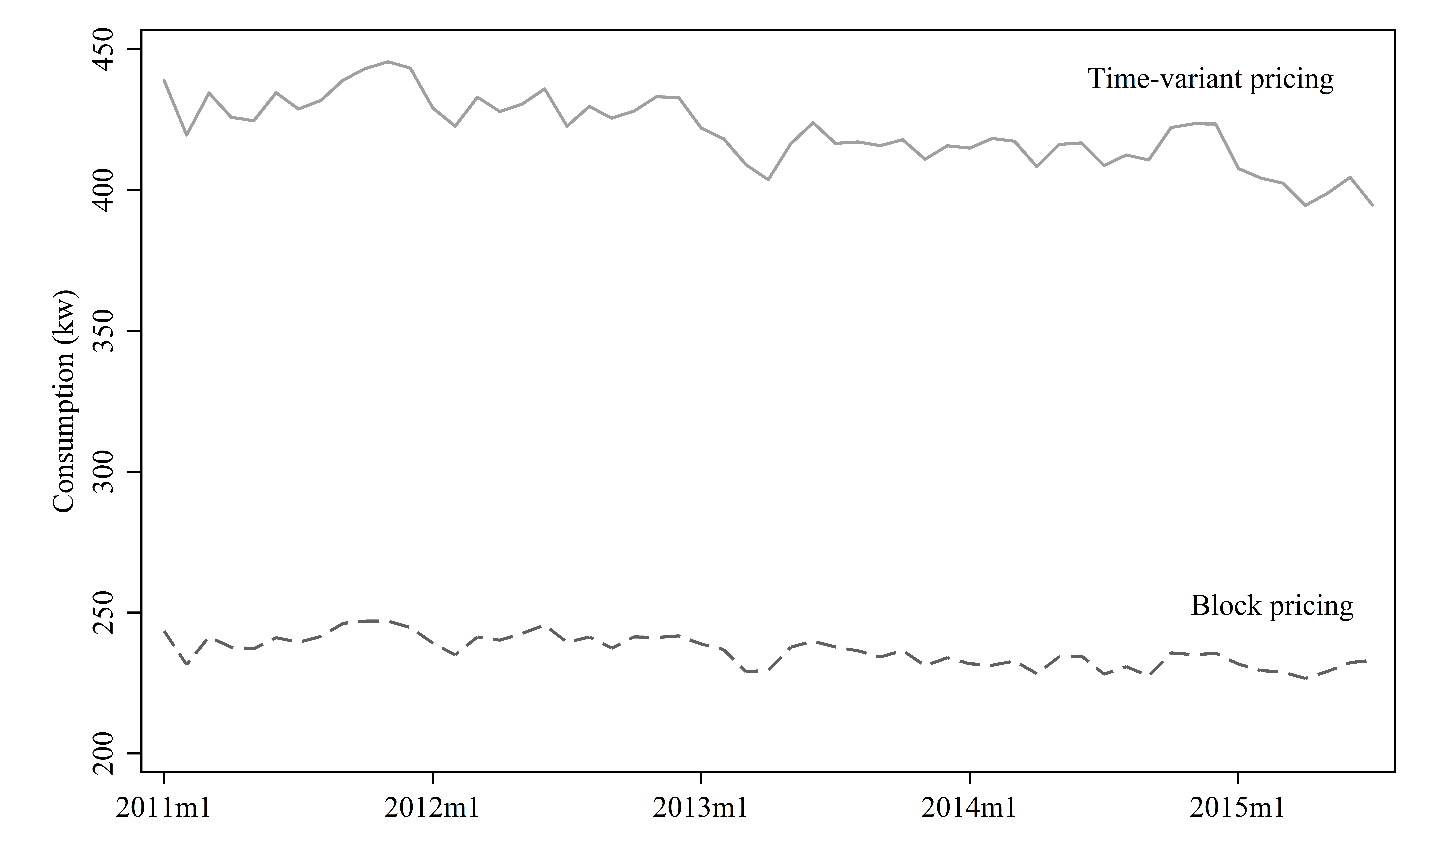
\includegraphics[width=1\textwidth]{./figures/image6.png}}
%   \end{center}
% \end{figure}
%
% \FloatBarrier
%
% \begin{figure}[ht]
%   \caption{Consumption by group and treatment status}\label{fig:seven}
%   \begin{center}
%   {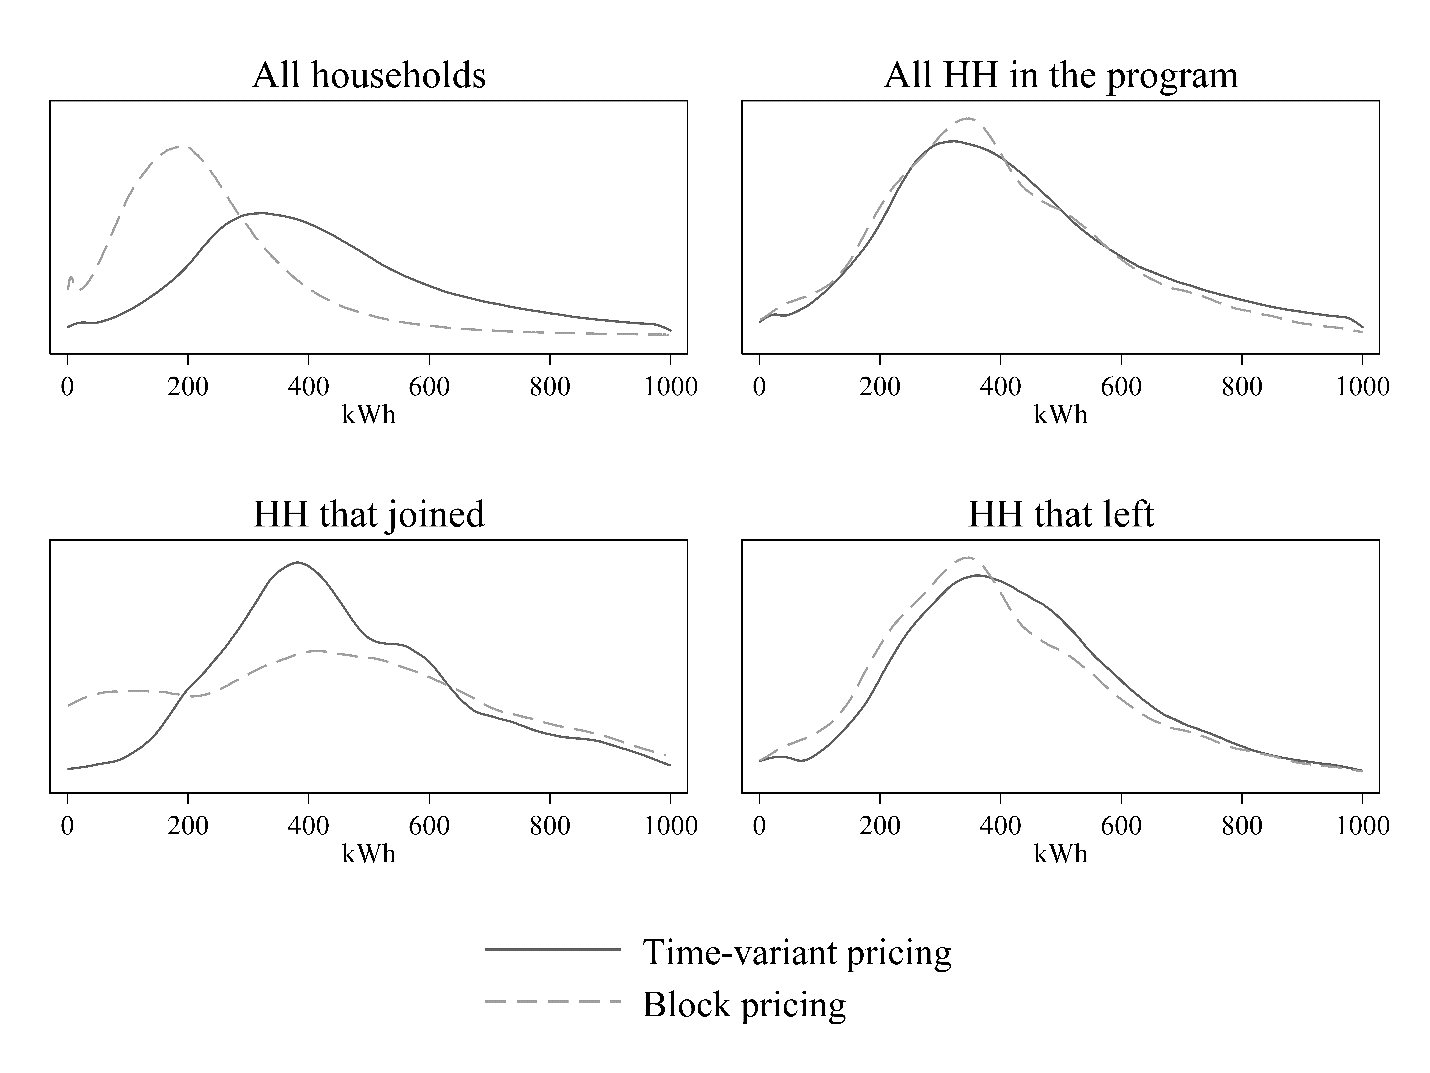
\includegraphics[width=1\textwidth]{./figures/image7.png}}
%   \end{center}
% \end{figure}
%
% Epanechnikov kernel densities comparing the consumption of different groups of households when they are in the TVP program and when they are not in the TVP program.
%
% \FloatBarrier

\clearpage

\subsection{Households that joined between 2011 and 2015}\label{appendix:B}
%
% \begin{figure}[ht]
%   \caption{Consumption trend after joining the program}\label{fig:eight}
%   \begin{center}
%   {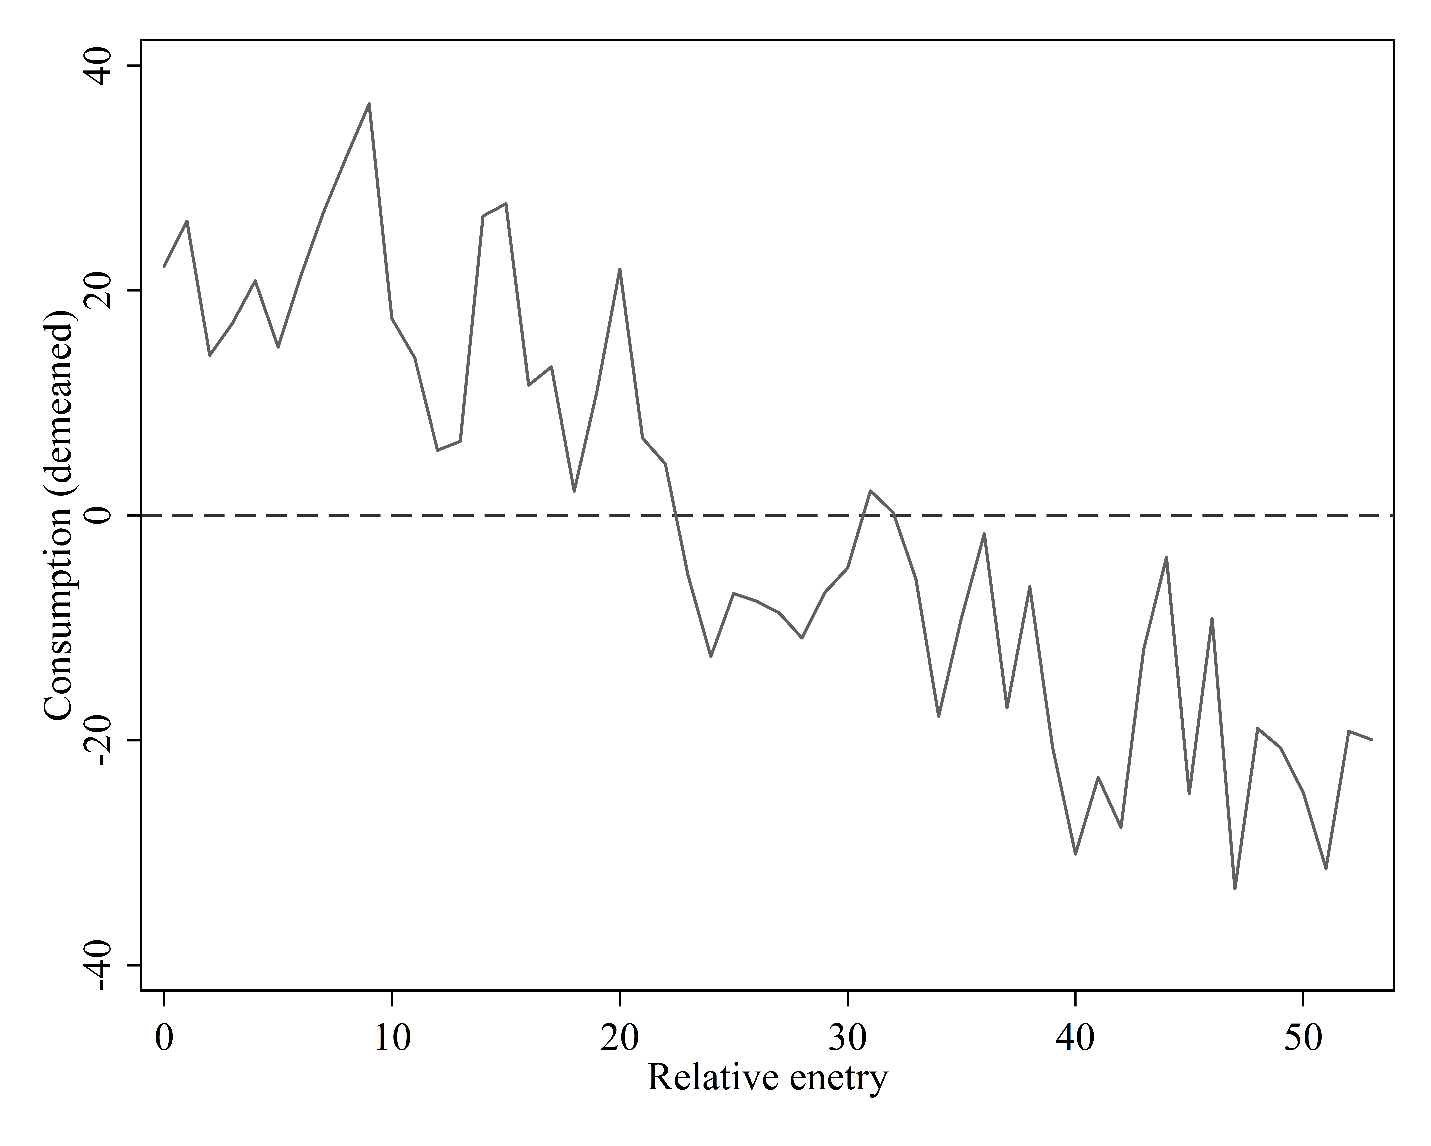
\includegraphics[width=1\textwidth]{./figures/image8.png}}
%   \end{center}
% \end{figure}
%
% Demeaned average monthly consumption after joining the TVP program.\par
%
% \FloatBarrier
%
% \begin{figure}[ht]
%   \caption{Number of households joining in each period}\label{fig:nine}
%   \begin{center}
%   {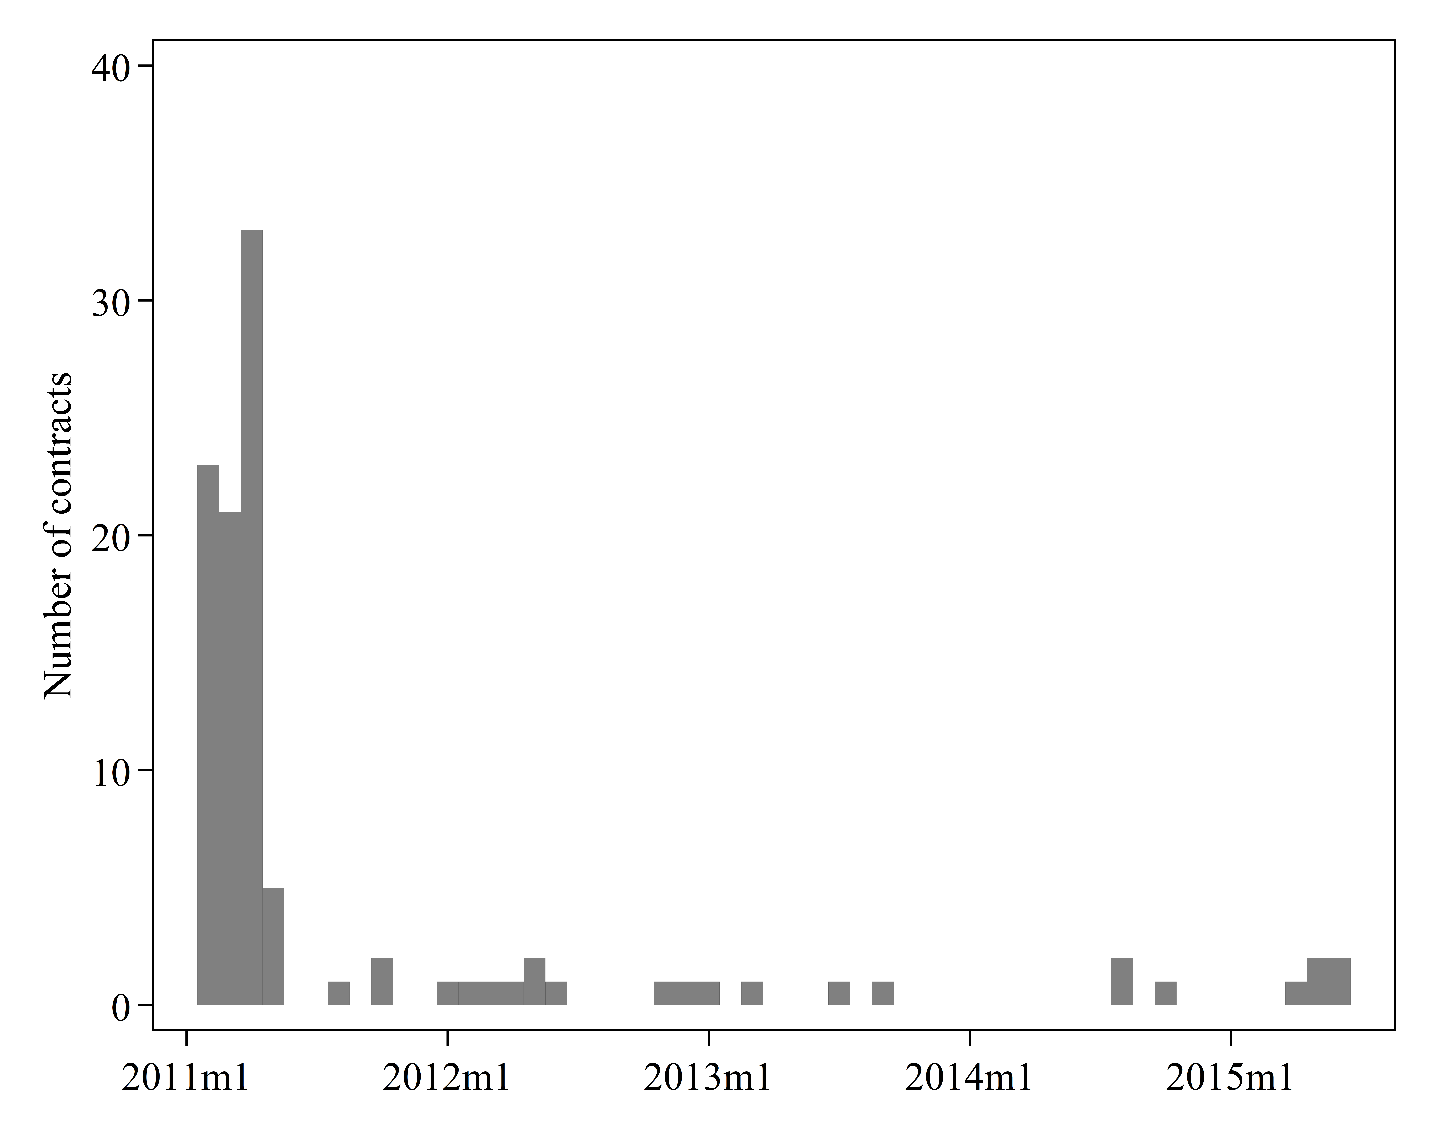
\includegraphics[width=1\textwidth]{./figures/image9.png}}
%   \end{center}
% \end{figure}
%
% \FloatBarrier
%
% \begin{figure}[ht]
%   \caption{Number of observations in each relative period}\label{fig:ten}
%   \begin{center}
%   {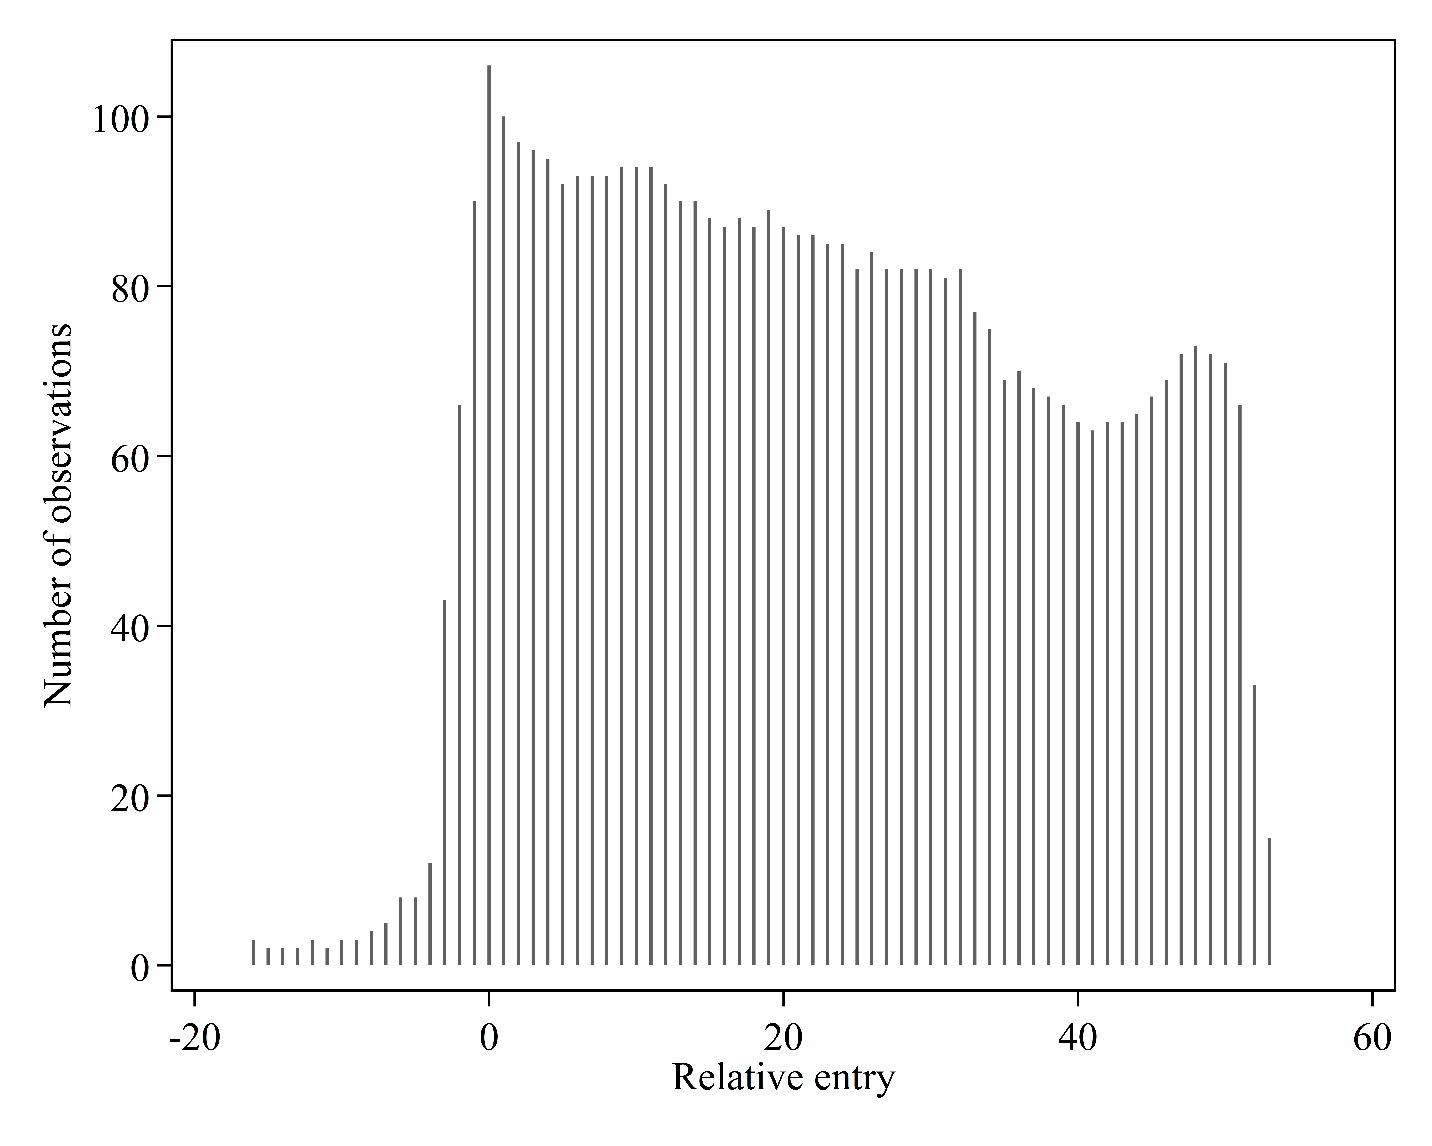
\includegraphics[width=1\textwidth]{./figures/image10.png}}
%   \end{center}
% \end{figure}
%
% \FloatBarrier
%
% \begin{figure}[ht]
%   \caption{Demeaned consumption by relative period}\label{fig:eleven}
%   \begin{center}
%   {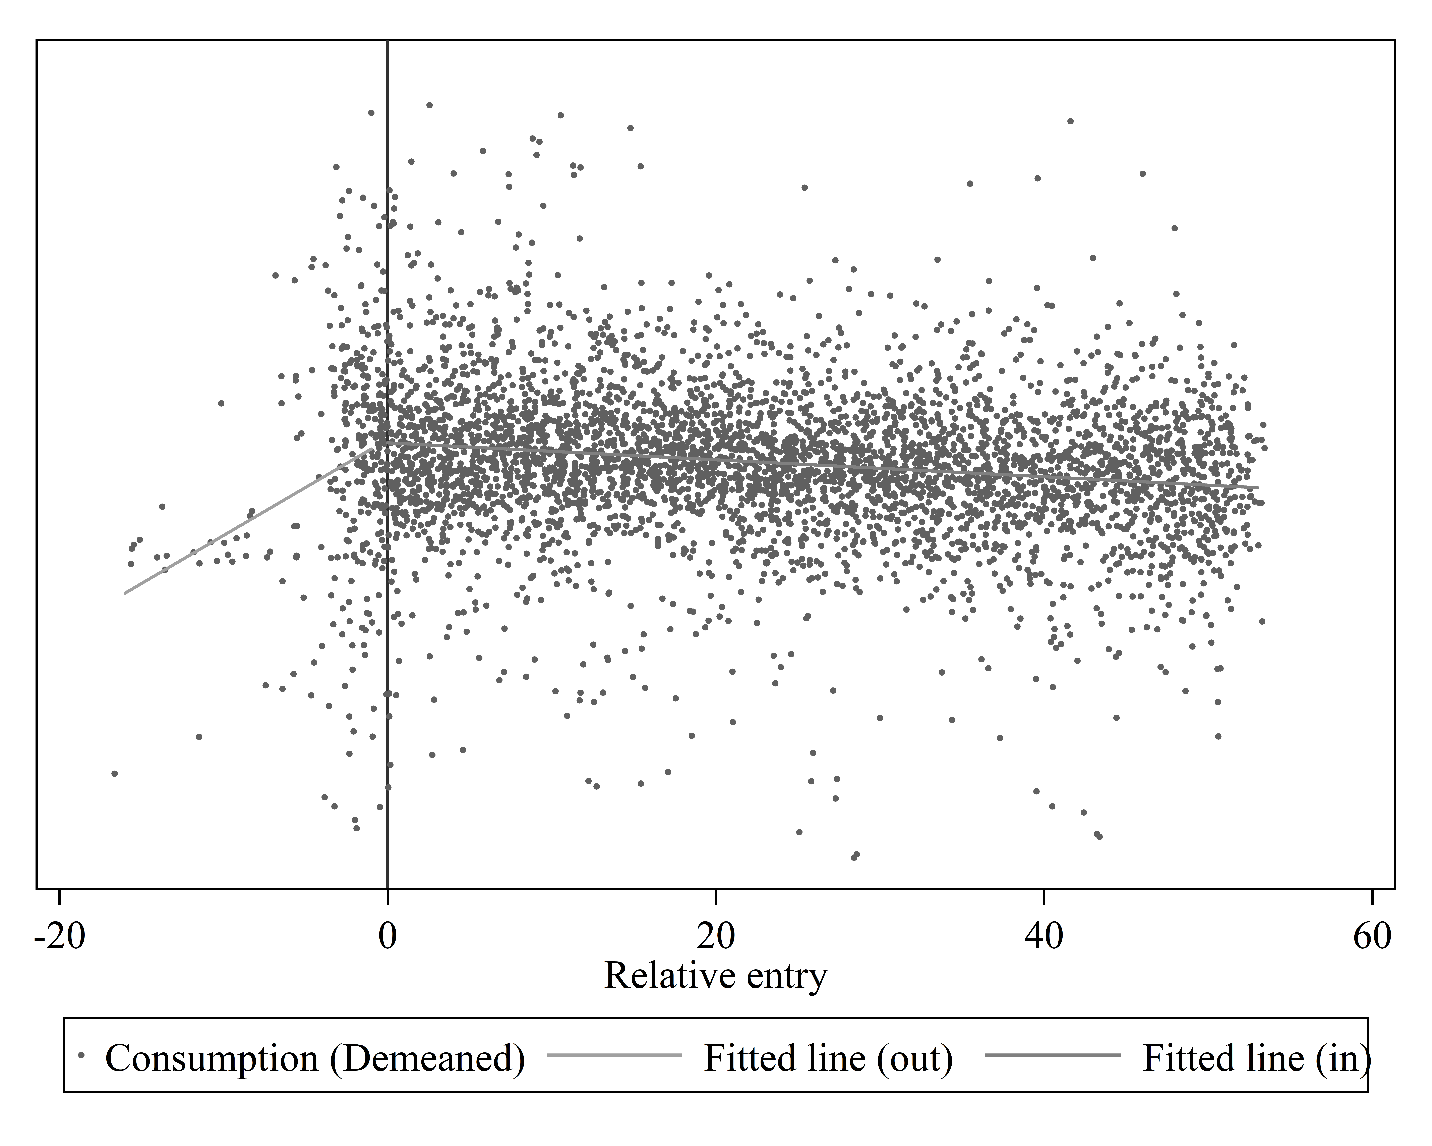
\includegraphics[width=1\textwidth]{./figures/image11.png}}
%   \end{center}
% \end{figure}
%
% \FloatBarrier

% \clearpage

\subsection{Households that left between 2011 and 2015}\label{appendix:C}
%
% \begin{figure}[ht]
%   \caption{Consumption trend before leaving the program}\label{fig:twelve}
%   \begin{center}
%   {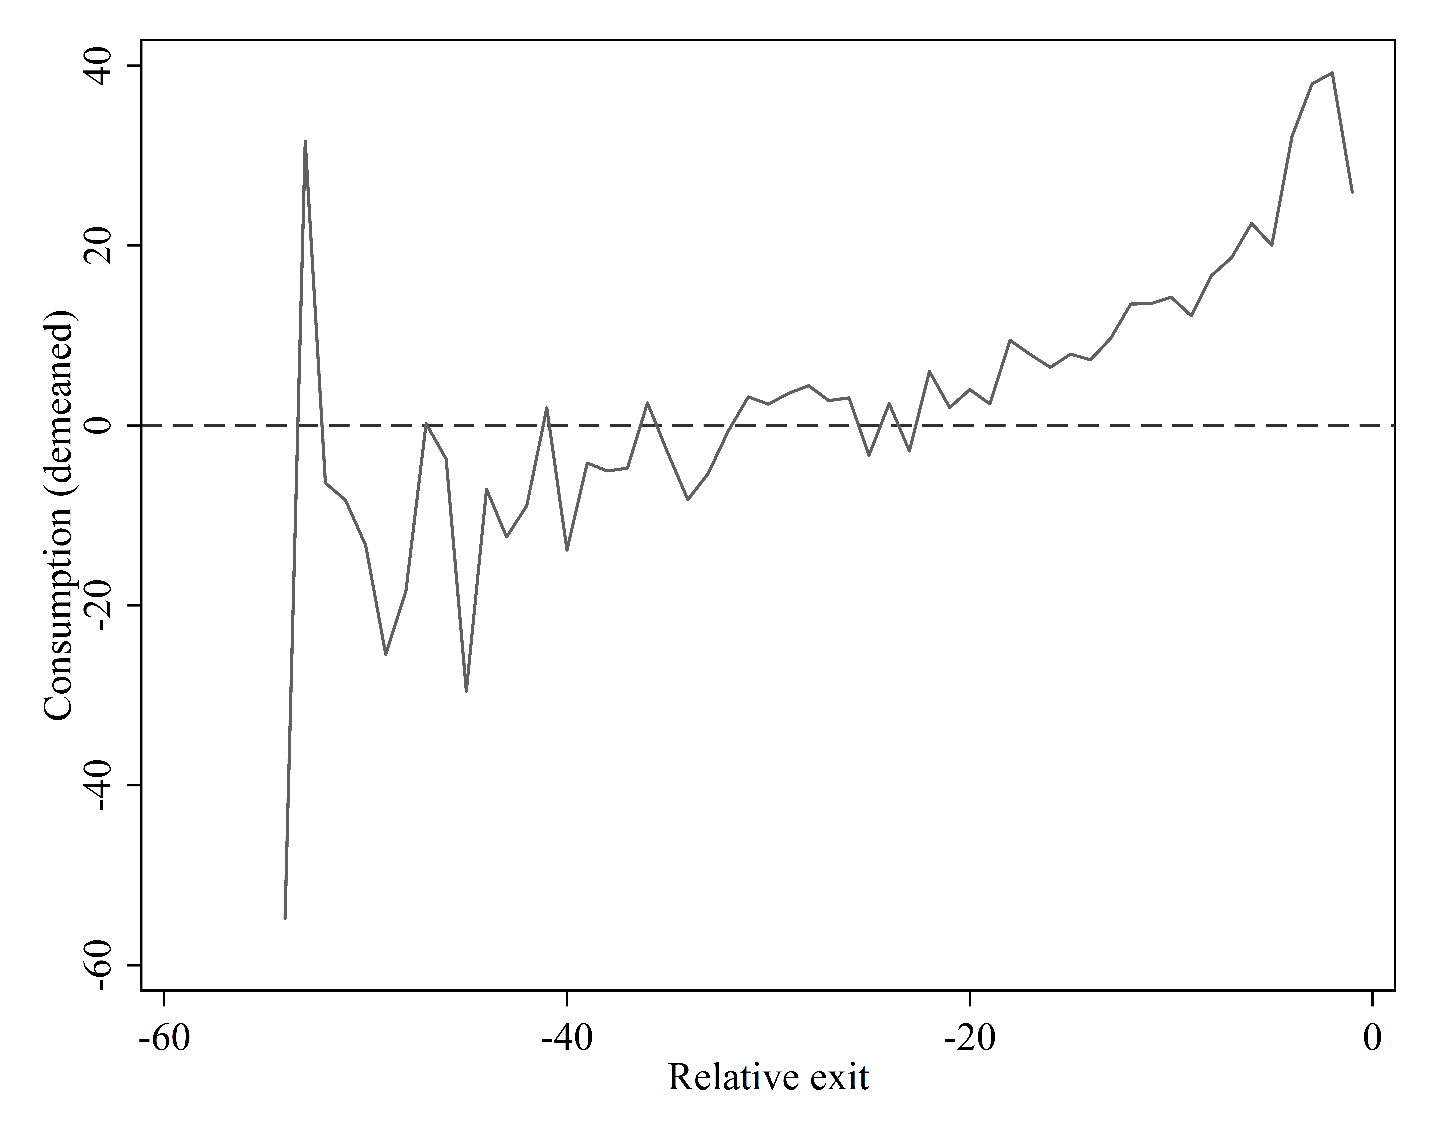
\includegraphics[width=1\textwidth]{./figures/image12.png}}
%   \end{center}
% \end{figure}
%
% Demeaned average monthly consumption before leaving the TVP program.\par
%
% \FloatBarrier
%
% \begin{figure}[ht]
%   \caption{Number of households leaving in each period}\label{fig:thirteen}
%   \begin{center}
%   {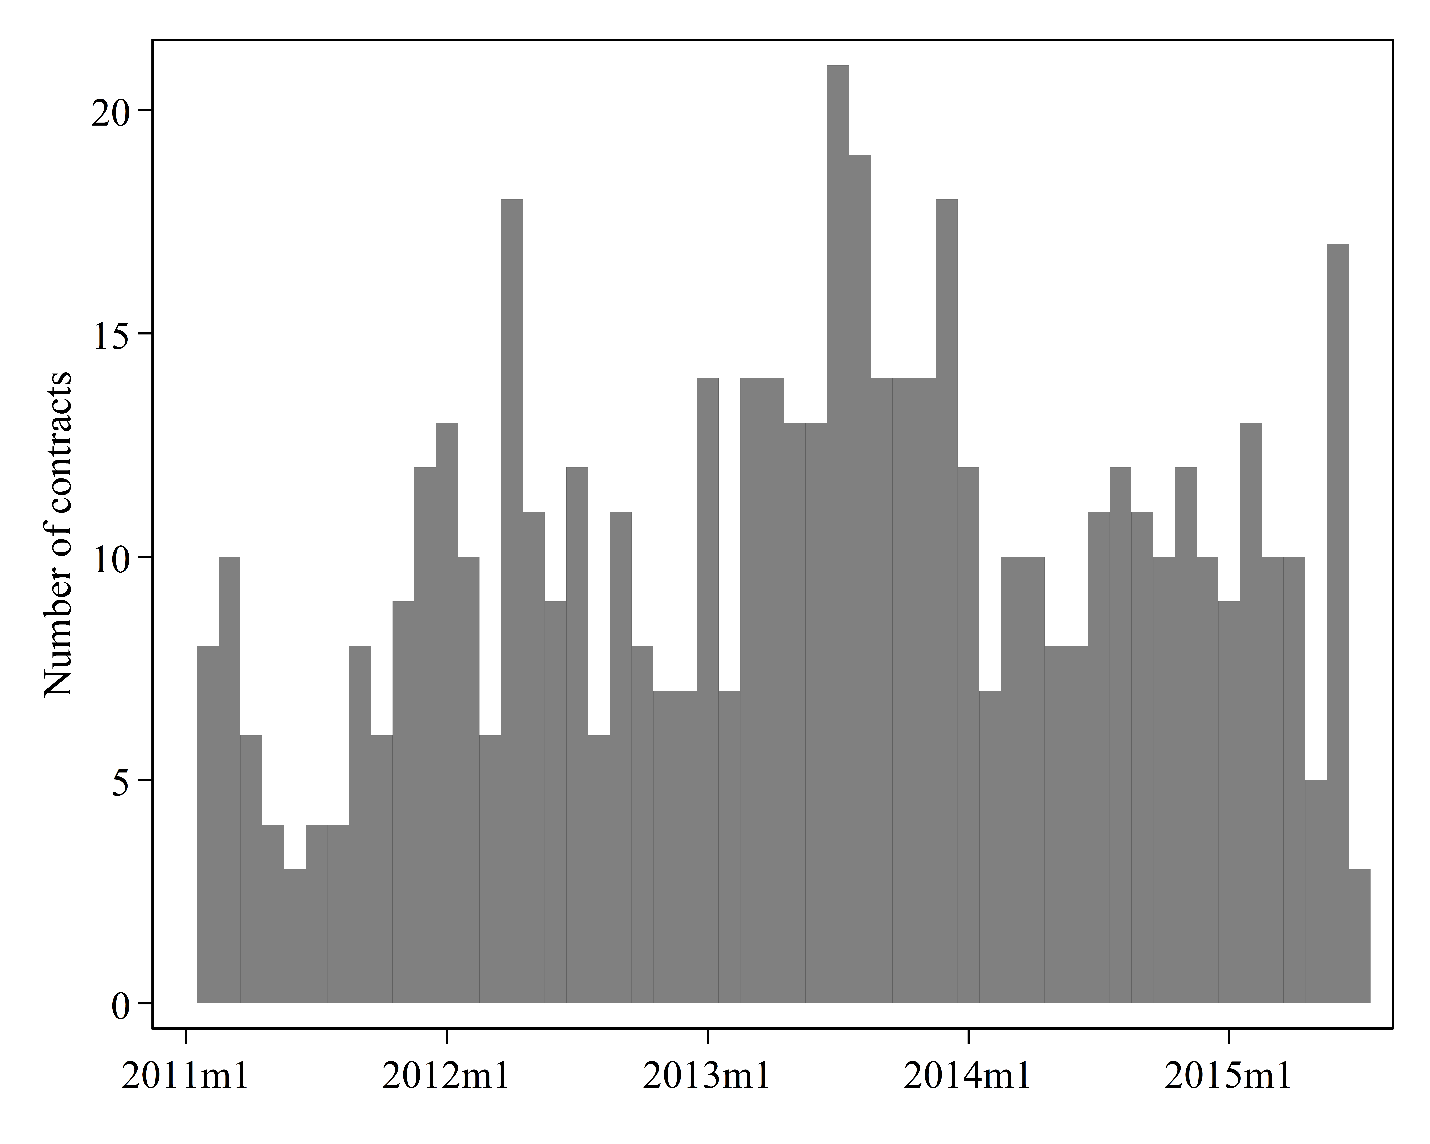
\includegraphics[width=1\textwidth]{./figures/image13.png}}
%   \end{center}
% \end{figure}
%
% \FloatBarrier
%
% \begin{figure}[ht]
%   \caption{Number of observations in each relative period}\label{fig:fourteen}
%   \begin{center}
%   {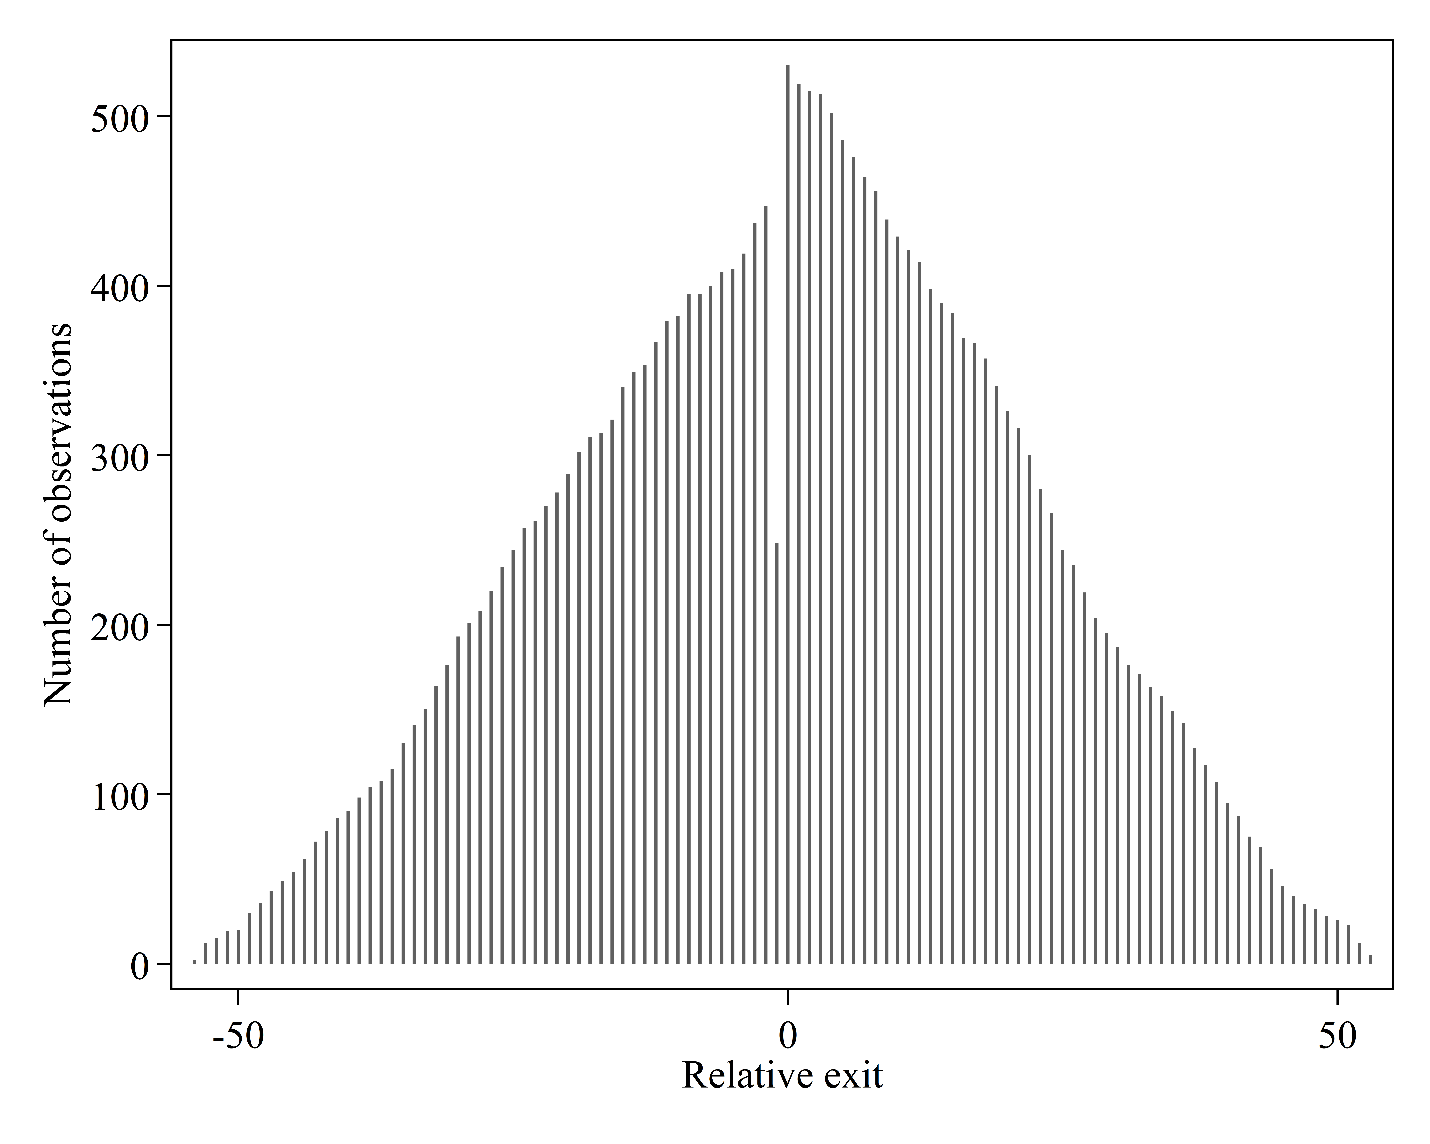
\includegraphics[width=1\textwidth]{./figures/image14.png}}
%   \end{center}
% \end{figure}
%
% The dip in the middle is explained by observations we dropped because the consumption data only covered a portion of the month.\par
%
% \FloatBarrier
%
% \begin{figure}[ht]
%   \caption{Demeaned consumption by relative period}\label{fig:fifteen}
%   \begin{center}
%   {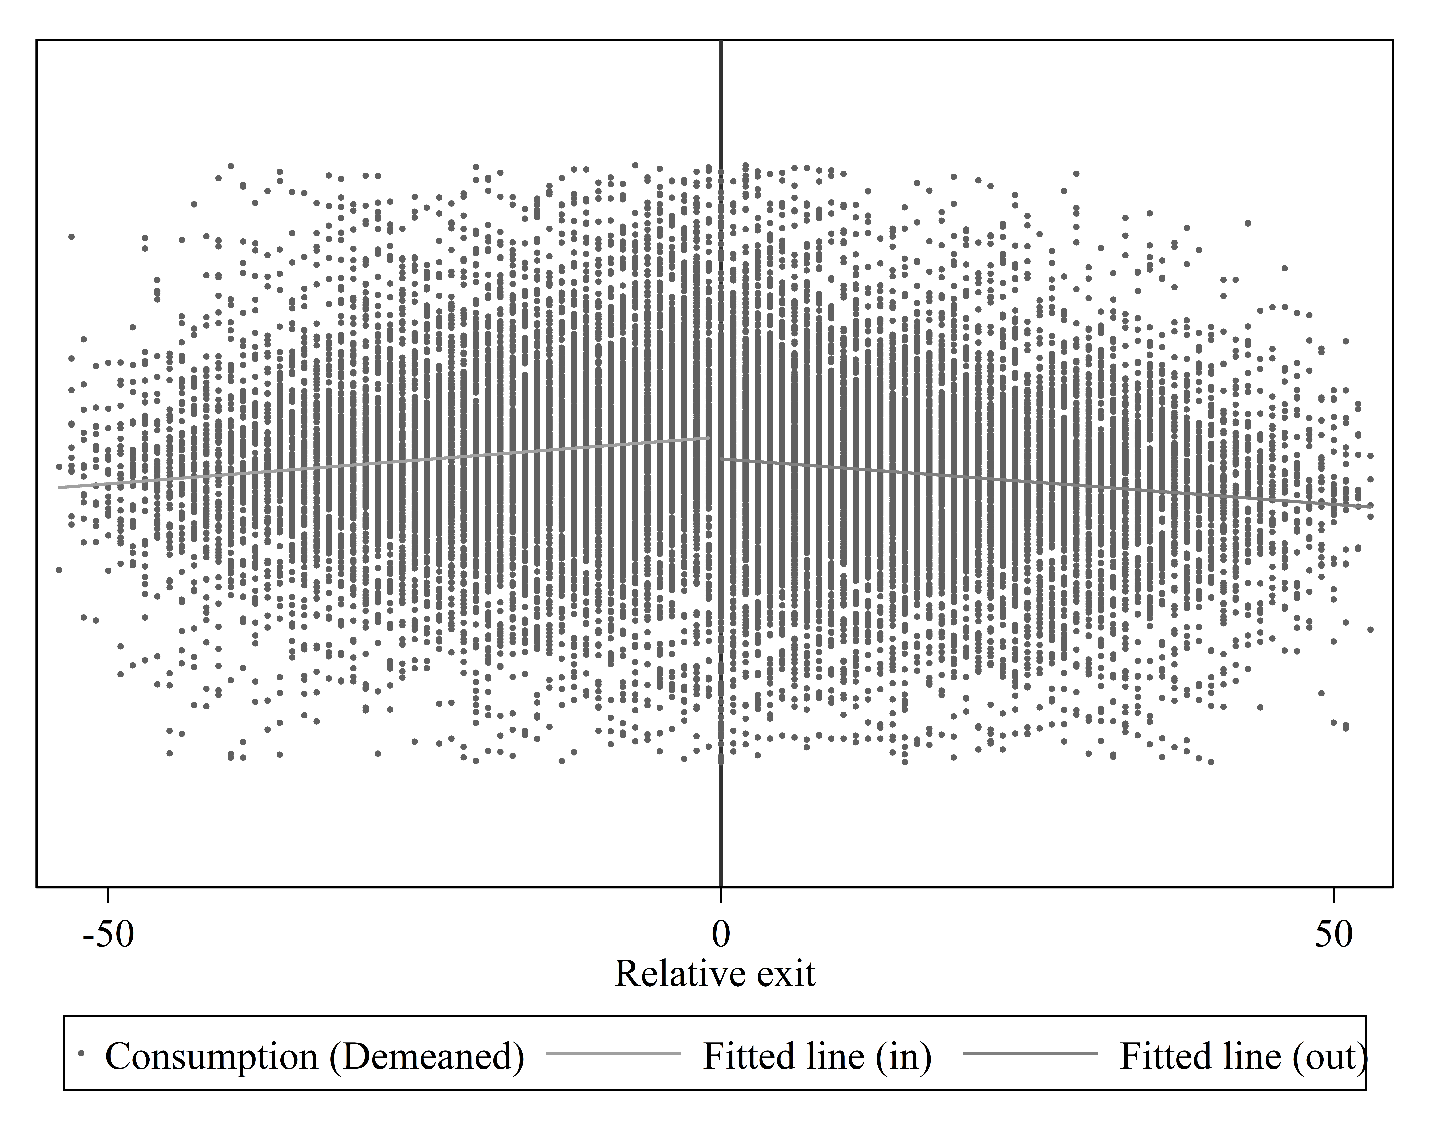
\includegraphics[width=1\textwidth]{./figures/image15.png}}
%   \end{center}
% \end{figure}
%
% \FloatBarrier
%
% \clearpage

% \subsection{Total consumption over time by type of households}\label{appendix:D}
%
% \begin{figure}[ht]
%   \caption{Total consumption over time by type of households}\label{fig:sixteen}
%   \begin{center}
%   {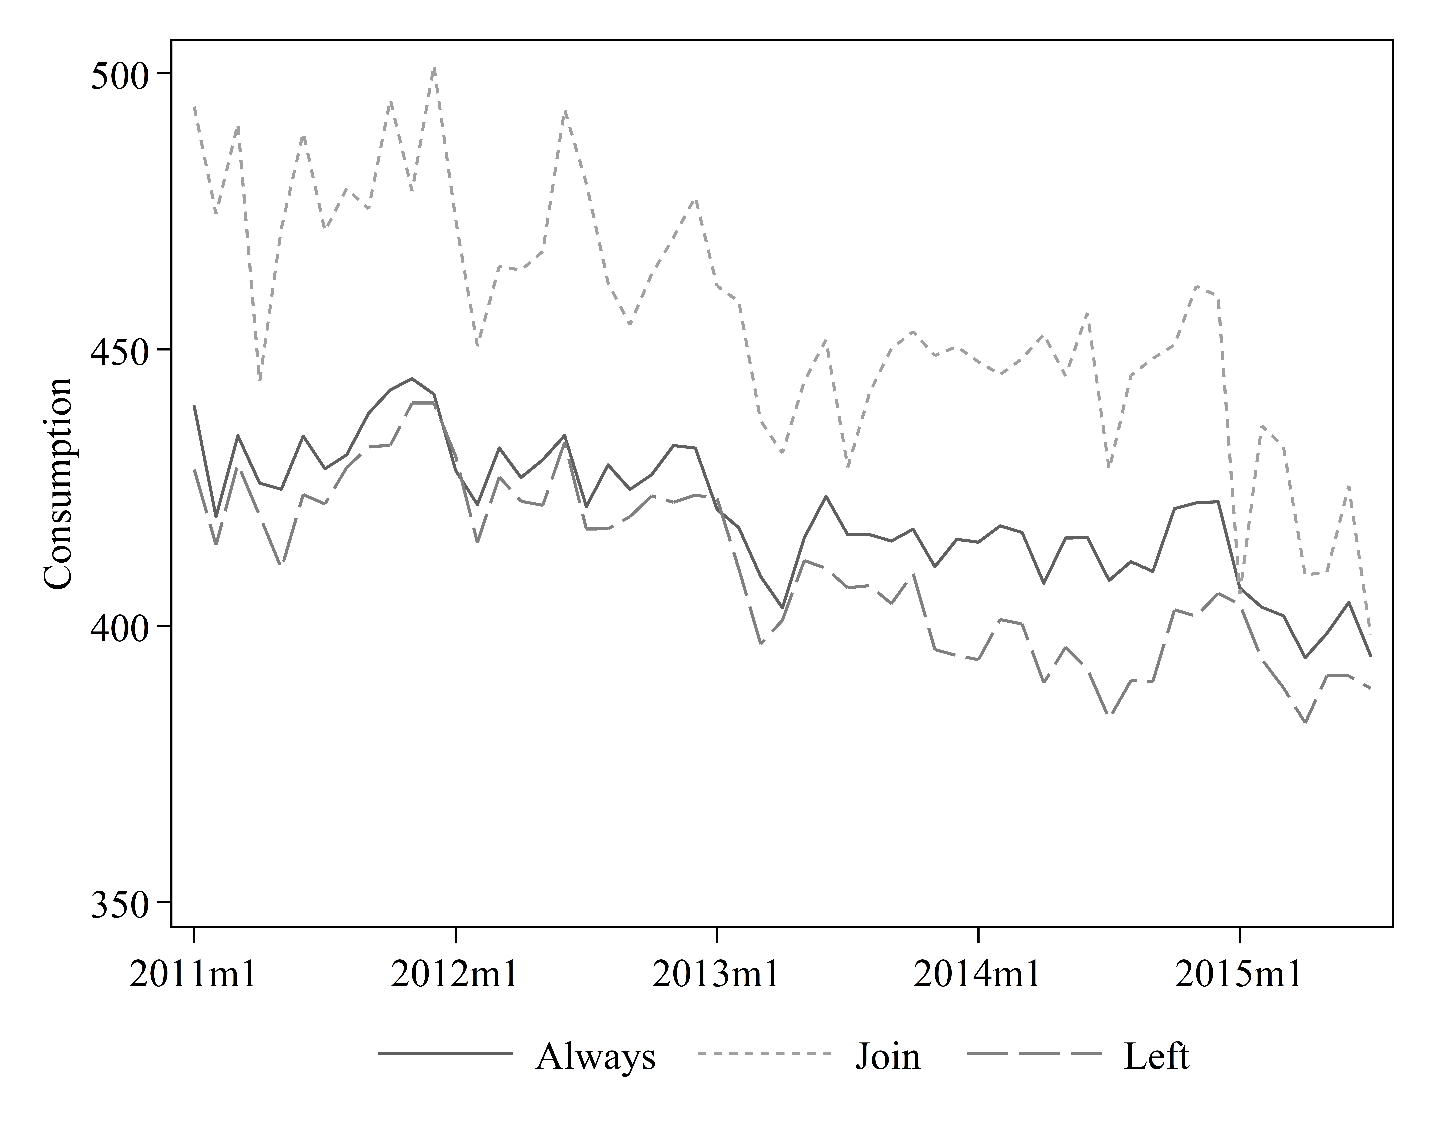
\includegraphics[width=1\textwidth]{./figures/image16.png}}
%   \end{center}
% \end{figure}
%
% \FloatBarrier
%
% \clearpage
%
% \subsection{The effect of TVP on peak consumption}\label{appendix:E}
%
% Estimating the effect of Time-Varying Pricing (TVP) on consumption during peak hours has been the focus of previous research. Here we provide suggestive evidence consistent with previous results: TVP is effective at reducing consumption during peak hours. Because we do not observe consumption data disaggregated by time of consumption when a household is not in the TVP program, we rely on a very strong assumption to provide graphical evidence of the effect of TVP on peak consumption. Explicitly, we use the fact that the time blocks – i.e., peak, mid-peak, and off-peak hours – were defined based on historical aggregate consumption data, and assume that the disaggregated consumption of household that were in the program for at least one period– groups  \( I \)  (only in the program),  \( J \)  (joined the program), and  \( L \)  (left the program) – was consistent with the definition of the time blocks \textit{when they were not in the program}. Since we assume the counterfactual, we do not have data to compare the actual disaggregated consumption. Instead, we rely on graphical evidence showing the disaggregated consumption over time by each type of household. In practice, under our identifying assumption, we say that if the consumption per hour during the peak-hour time block is not the highest, the program was successful in reducing consumption during the peak hours. This result holds unless the differences in consumption patterns between the general population and the self-selected group that participated in the TVP program are such that the self-selected groups do not consume the most during peak hours when not in the program.
%
% Figure E1 shows our graphical evidence. In the top panel, for households that were always in the program, the hourly consumption during mid-peak hours is the highest, closely followed by the hourly consumption during peak hours, and the consumption during off-peak hours is the lowest. Also, there seems to be a seasonal pattern around the end and beginning of the year in which hourly consumption during peak hours is higher than during mid-peak hours. Overall, the consumption for all time blocks for this group of households is smooth, which might imply that households have been in the program for enough time and are not adjusting their consumption any further in response to the earlier change\ of pricing schedule. We observe the same patterns for households that joined during 2011 and 2015, but hourly consumption is not as smooth as in the previous case. Still, the gap from mid and peak hourly consumption is increasing in a way that might eventually converge to the patterns observed for the households that were always in the program. Finally, for the households that left the program between 2011 and 2015, it is hard to distinguish between the hourly consumption during peak and mid-peak hours.  Under our identifying assumption, we conclude that the graphical evidence is suggestive of success of the policy in reducing consumption during peak hours.
%
% \begin{figure}[ht]
%   \caption{Disaggregated consumption by type of household}\label{fig:seventeen}
%   \begin{center}
%   {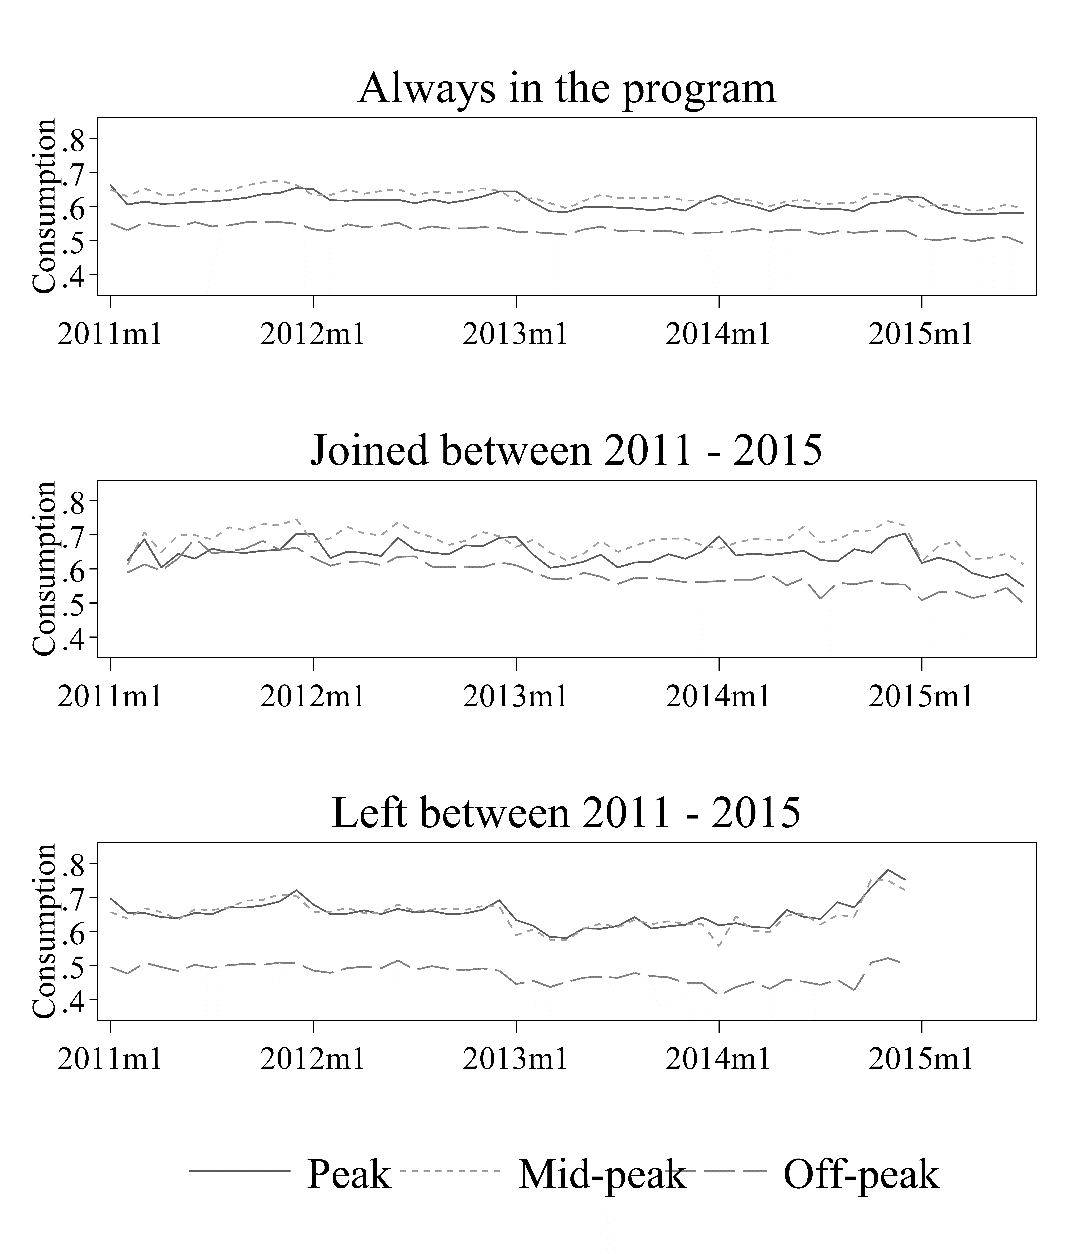
\includegraphics[width=1\textwidth]{./figures/image17.png}}
%   \end{center}
% \end{figure}
%
% \FloatBarrier
%
% \begin{figure}[ht]
%   \caption{Consumption over time by time block and type of contract}\label{fig:eightteen}
%   \begin{center}
%   {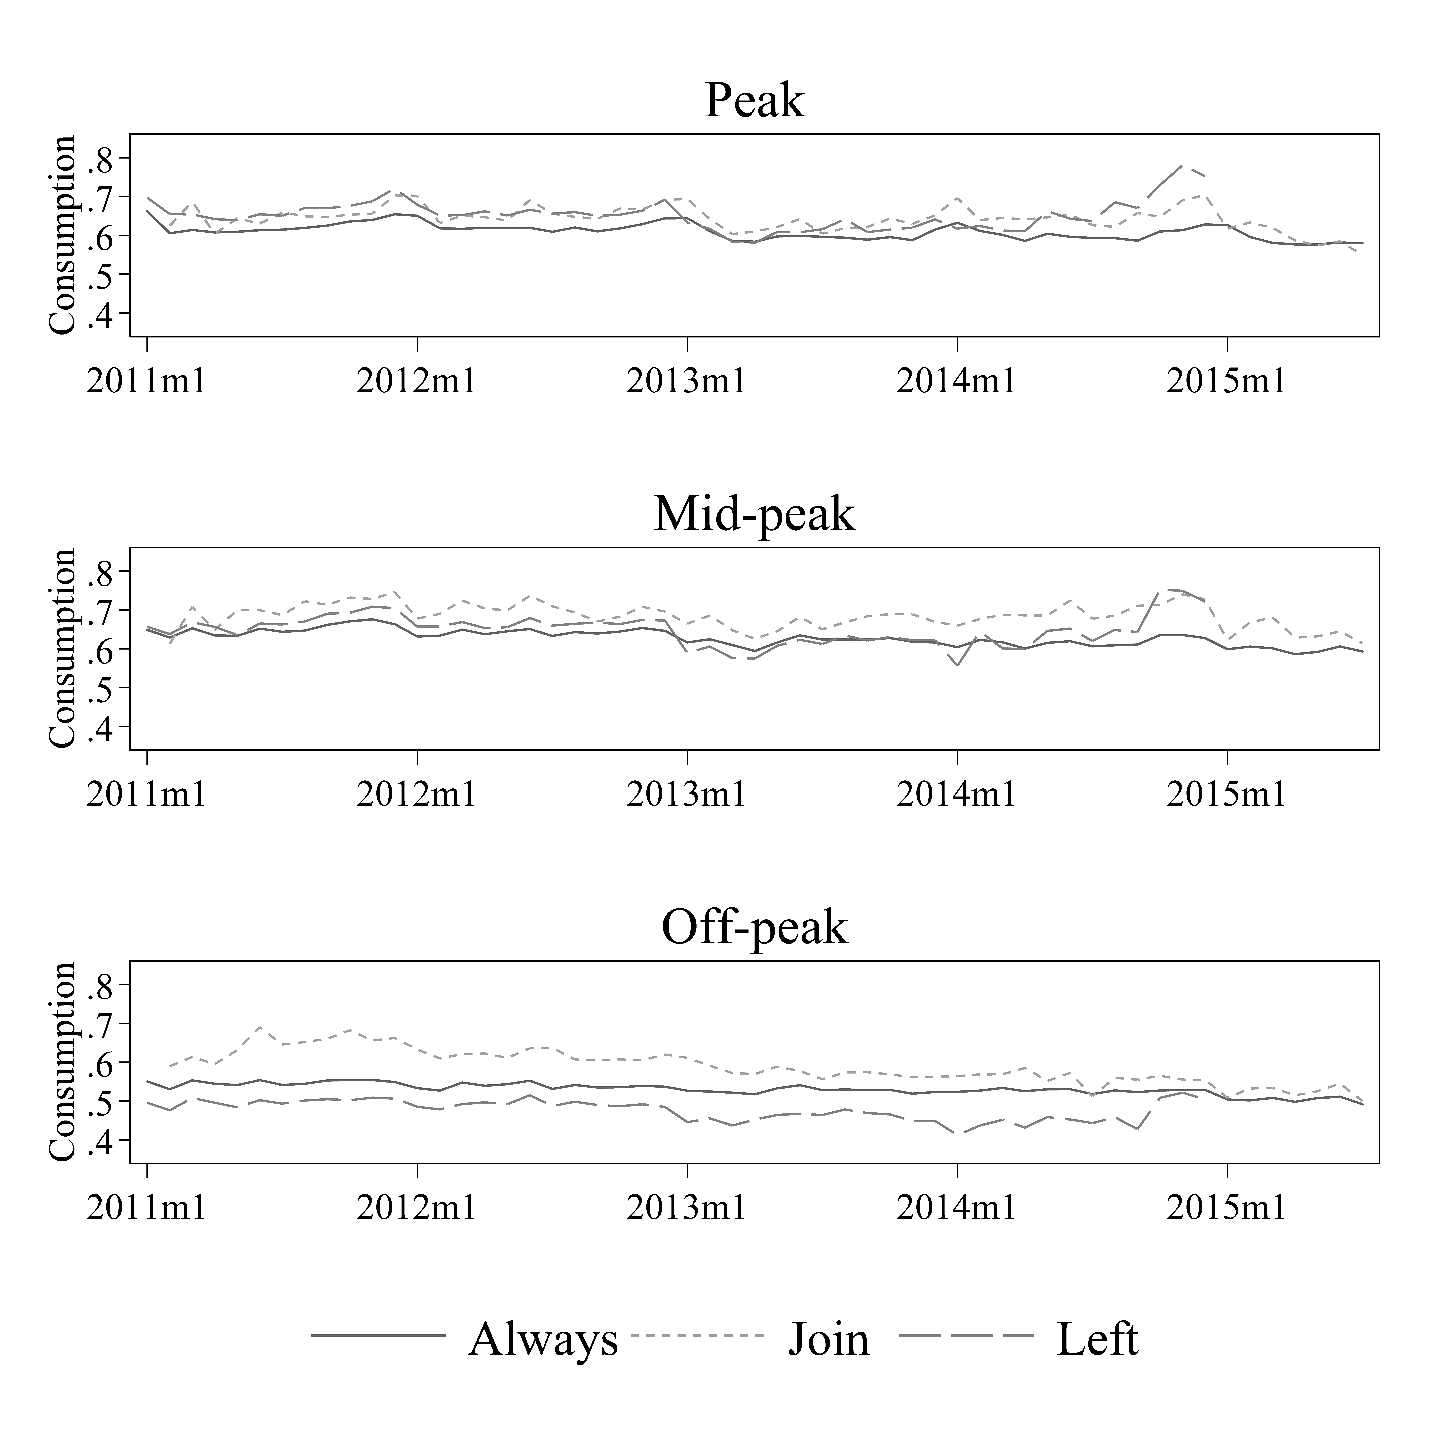
\includegraphics[width=1\textwidth]{./figures/image18.png}}
%   \end{center}
% \end{figure}
%
% \FloatBarrier
%
% \clearpage

\subsection{Bunching}\label{appendix:F}
%
% \begin{figure}[ht]
%   \caption{Bunching}\label{fig:nineteen}
%   \begin{center}
%   {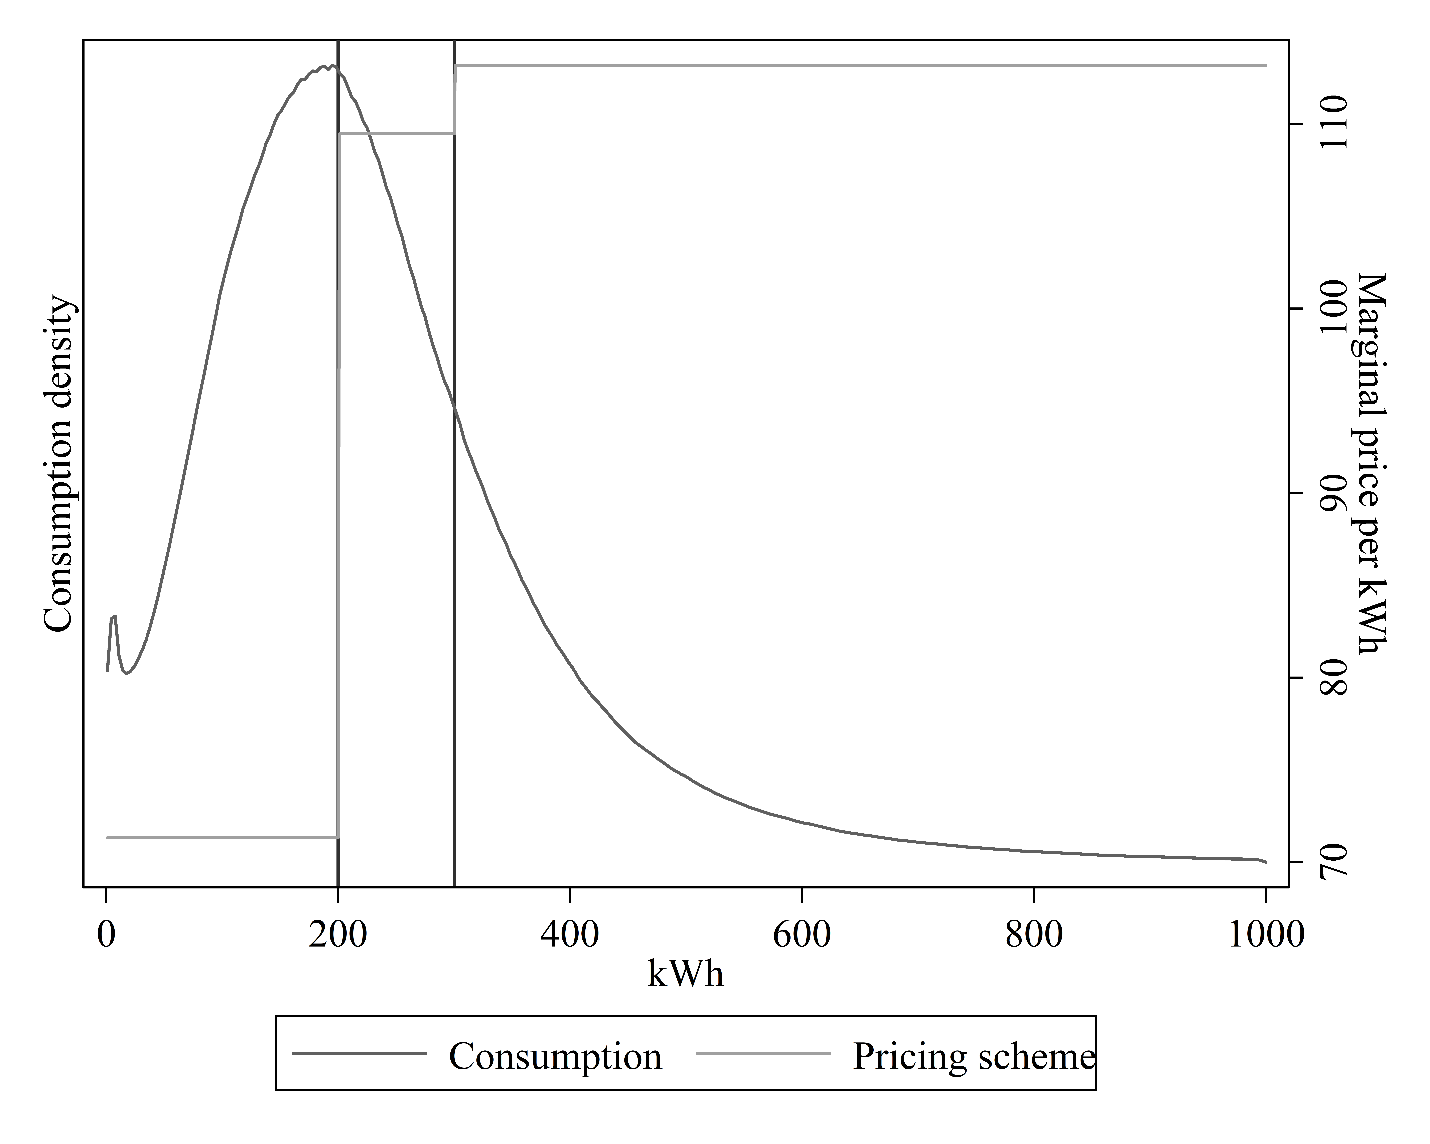
\includegraphics[width=1\textwidth]{./figures/image19.png}}
%   \end{center}
% \end{figure}
%
% \FloatBarrier
